\section{Model vodenja razvit z genetskim algoritmom} \label{genetski}

Če je ovčar čredi preblizu, se ovce razkropijo, če je predaleč, pa jih ne more voditi. Najboljša razdalja je odvisna od števila ovc. Prav tako verjetno obstajajo tudi boljše vrednosti preostalih parametrov modela (tabela~\ref{table:ovcar}) v odvisnosti od števila ovc, ovčarjev in modela gibanja ovc.

Ker je ročno razviti model pogosto neuspešen, si želimo najti optimalne vrednosti parametrov. Za vsak parameter lahko postavimo neke smiselne meje, kjer bi ta vrednost lahko bila. Ker je dobljeni prostor (produkt 21 intervalov, največja hitrost je konstantna) prevelik, moramo najti nek način iskanja najboljših vrednosti v tem prostoru. Četudi bi zvezne intervale razdelili na le 10 diskretnih vrednosti, bi morali preveriti $10^{21}$ kombinacij vrednosti parametrov. Če bi le vrnili ničelni izhod, bi en računalnik s 16 jedri in hitrostjo procesorja 3,5 GHz preverjal vse kombinacije več kot 580 let. Torej nam tu ne bi pomagala niti uporaba več računalnikov, saj nikakor ne bi zaključili vseh potrebnih simulacij v nekem doglednem času.

Odločili smo se za pristop z genetskim algoritmom, ki temelji na ideji naravne selekcije pri evoluciji v naravi. Genetski algoritmi so populacijski algoritmi za optimizacijske probleme. Ker je algoritem vseeno zamuden, smo simulacijo omejili na 3 minute (omejeno s številom korakov simulacije, ki ustrezajo 3 minutam in ne z dejanskim časom izvajanja) in jo nato prekinili, če se simulacija še ni sama zaključila z uspešnim izidom. Pri implementaciji smo se zgledovali po podrobni razlagi algoritma v~\cite{natureOfCode}.

Ideja genetskih algoritmov je ta, da imamo začetno populacijo naključnih genov, tej začetni generaciji pa sledijo generacije, ki naj bi bile sčasoma v povprečju vedno boljše. Pri tem moramo dobro definirati, kaj je gen in kaj pomeni, da je nek gen "boljši".

\subsection{Gen in evalvacija uspešnosti gena}

Vsak osebek v populaciji ima določene vrednosti vseh 21 parametrov in temu zaporedju števil pravimo gen. Tako je na primer genotip za hitrost ovčarja v stanju vodenja pri ročno razvitem modelu enak 2/3 (le numerična vrednost), fenotip pa je njegova izražena hitrost v stanju vodenja 5 m/s. Opazimo, da se med evolucijo lahko pojavi tudi gen, ki ustreza fenotipu ročno razvitega ovčarja. Ob koncu evolucije torej lahko pričakujemo vsaj tako dober ali celo boljši gen in s tem večjo uspešnost vodenja, saj bi tudi ročno razviti model izumrl, če ne bi bil vsaj primerljiv z najboljšim genom.

Da evolucija deluje dobro, mora biti v začetnem genomu dovolj različnih genov. Če geni niso dovolj različni, bodo naslednje generacije preveč podobne prvi in odvisne od začetka simulacije. Če pa genov ni dovolj, se lahko hitro izgubi potencial, ki se skriva v posameznem genu.

Uspešnost posameznega gena moramo za potrebe simuliranja naravne selekcije nekako oceniti. Za ocenjevanje uspešnosti gena potrebujemo cenilko uspešnosti za evalvacijo gena. Pri tem upoštevamo čas potreben za simulacijo (zadnja ovca v staji), število ovc na pašniku ob koncu simulacije, oddaljenost preostanka črede od staje in čase prihodov v stajo. Funkcija naj bi bila konveksna v primeru, ko je pomembna dejanska ocenjena vrednost in ne le razvrstitev med ostalimi geni.

Naša izbrana funkcija za oceno uspešnosti posamezne simulacije je
\begin{align}
\phi(N, (t_j)_{j_1}^k, \mathbf{GCM}) &= 210\Big(\frac{t_{MAX} - t_N}{t_{MAX}}\Big)^2\frac{1}{N}\sum_{j=1}^k \frac{t_{MAX} - t_j}{t_{MAX}} \label{eq:genetski} \\
 &+ \frac{1}{1 + N - k + (N - k)\Vert \mathbf{GCM} - \mathbf{F}\Vert}, \nonumber
\end{align}
kjer je $t_{MAX}$ časovna omejitev simulacije v sekundah, $N$ začetno število ovc, $k$ število ovc pripeljanih v stajo in $\mathbf{F}$ lokacija staje. Po tej formuli dobimo večjo uspešnost za simulacije, ki prej v stajo pripeljejo večji delež črede. Tako je bolj uspešen gen, kjer je zadnja ovca prej v staji. Nekoliko manj pomembno je, da so bile ovce v povprečju prej pripeljane v stajo oziroma, da nam je ostal večji delež časa. Faktor 210 služi le normalizaciji, da je želena uspešnost med 0 in 100. Ker pa je v primeru $t_N = t_{MAX}$, ko je na pašniku še vsaj ena ovca, prvi člen enak 0, mu prištejemo še drugi člen, kjer je pomembno število preostalih ovc na travniku in je še nekoliko manj pomembna razdalja med GCM in F. S tem lahko po uspešnosti razvrstimo tudi simulacije, kjer je na pašniku ostala še vsaj ena ovca.

\subsection{Nova generacija}

Ko ocenimo uspešnost vseh genov v generaciji, moramo narediti novo generacijo, kjer damo večjo verjetnost za ponovno pojavitev genom, ki jim je šlo bolje. Pri tem pa moramo ohranjati dovoljšnjo variabilnost genoma.

Genetski algoritem sestoji iz več generacij. Novo generacijo naredimo iz prejšnje z uporabo selekcije, kjer imajo bolj uspešni geni večjo verjetnost parjenja, križanja obeh genov iz para in mutacij na dobljenem genu. Oglejmo si podrobnosti teh korakov. Na sliki~\ref{fig:genetski} lahko vidimo grafični prikaz razmnoževanja.

\begin{figure}[ht]  % ali t za na vrhu ali h! za točno tukaj
	\centering
	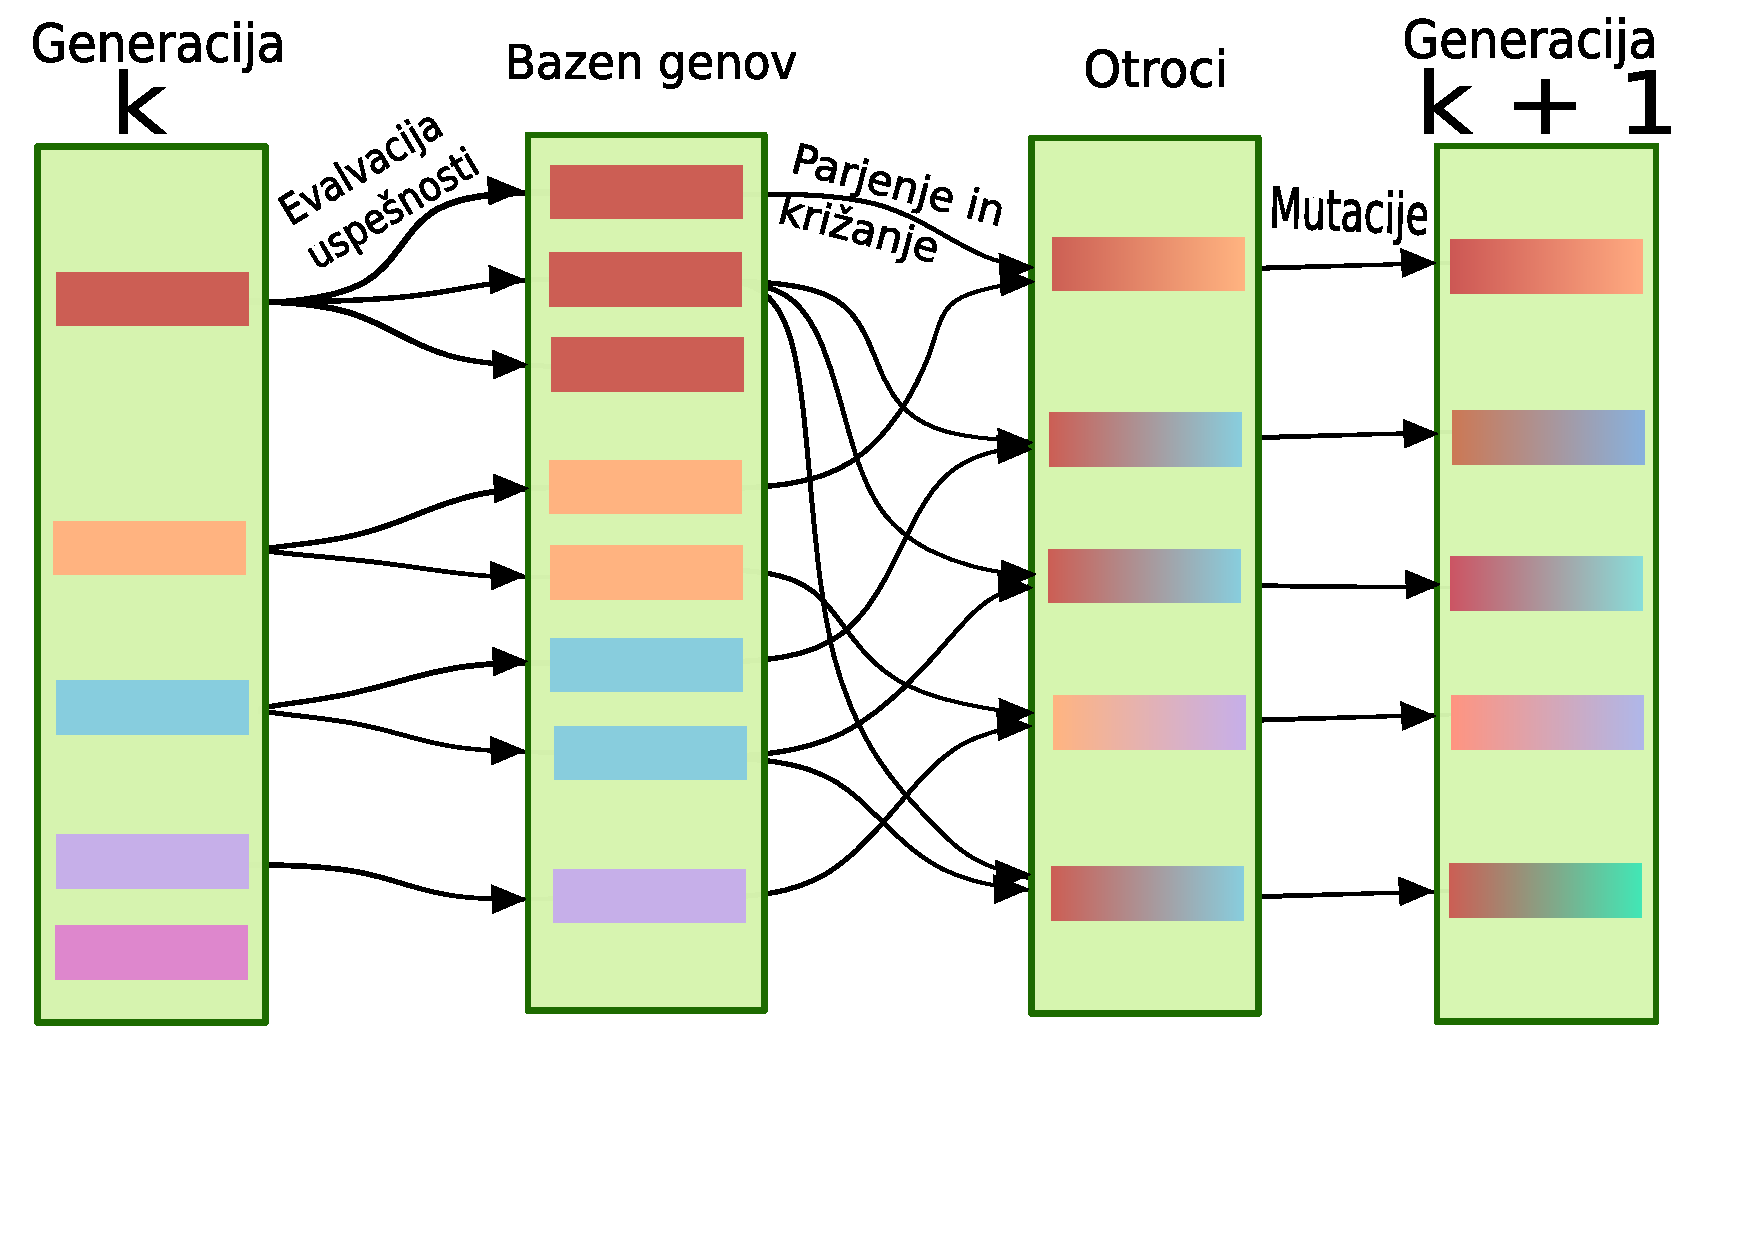
\includegraphics[width=0.9\textwidth]{../poglavja/images/genetski.pdf}
	\caption[Razmnoževanje uspešnejših genov]{Najprej geni z izmerjeno uspešnostjo (vhod), več ponovitev v bazenu bolj uspešnim, parjenje, križanje in mutacije (izhod).} % narejena je s programom Inkscape
	\label{fig:genetski}
\end{figure}

\subsubsection{Parjenje} \label{parjenje}

Obstaja mnogo različnih načinov parjenja. Lahko določimo, koliko najboljših genov se bo z enako verjetnostjo razmnoževalo, čemur rečemo elitna metoda, a tu se del genov ne pojavlja več v naslednjih generacijah razen v primeru mutacij. Mi smo si izbrali verjetnostni pristop, kjer ima vsak gen verjetnost parjenja odvisno od uspešnosti.

Za ta namen pripravimo bazen genov, iz katerega kasneje dobimo naključne pare. Pri tem v bazen postavimo $2 i^2 / n$ kopij gena (zaokroženo na najbližje celo število) z $i$-to najnižjo uspešnostjo, če imamo do konca evolucije še vsaj tri generacije, kjer je $n$ velikost populacije v eni generaciji. V zadnjih treh generacijah smo v bazen postavili $2 i^3 / n$ kopij $i$-tega gena, s čimer smo naredili še večji pritisk na naravno selekcijo, saj imajo slabši posamezniki še manjše možnosti za parjenje, s čimer je pristop na nek način bolj podoben elitni metodi. Na sliki~\ref{fig:verjetnost-parjenja} si lahko ogledamo verjetnosti za parjenje v seznamu genov razvrščenem po uspešnosti.

\begin{figure}[ht]  % ali t za na vrhu ali h! za točno tukaj
	\centering
	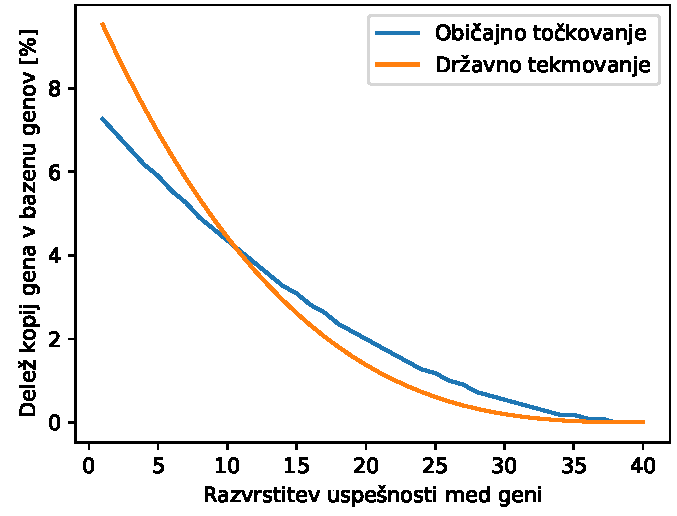
\includegraphics[width=0.5\textwidth]{../poglavja/images/parjenje.pdf}
	\caption[Verjetnost parjenja]{Graf z obema krivuljama.} % narejena je s programom Inkscape
	\label{fig:verjetnost-parjenja}
\end{figure}

Iz dobljenega bazena vzamemo $n$ parov genov.

\subsubsection{Križanje}

Vsak par genov naključno križamo in s tem dobimo večjo variabilnost genov v populaciji. Uveljavljenih je več pristopov križanja. Ker želimo ohranjati dolžino gena, se osredotočimo le na rezanje obeh genov v istih točkah in na uniformno izbiro. Križanje z rezanjem pomeni, da v eni ali dveh točkah prerežemo oba gena in nato vrnemo gen, kjer se izmenjujejo kosi, ki prihajajo od obeh staršev. Ker pa sosednost znotraj gena nič ne pomeni, smo se odločili za uniformno križanje, kjer naključno vsako vrednost iz zaporedja v nov gen kopiramo od enega ali drugega izmed staršev. Tako se gena enakomerno premešata.

\subsubsection{Mutacija}

Da ohranjamo raznolikost genoma in se s tem izogibamo lokalnim optimumom, dobljenemu genu na vsakem mestu z verjetnostjo $p$ izberemo novo naključno vrednost. Pri tem na vsakem koraku naredimo ožji interval, s katerega vrnemo naključno vrednost. S tem sčasoma dovoljujemo le še manjše spremembe, saj preveč mutacij lahko onemogoča evolucijski napredek skozi generacije. Vrnemo naključno vrednost z intervala $\lbrack x - \frac{1}{generacija} (M - m), x + \frac{1}{generacija} (M - m)\rbrack \cap \lbrack m, M \rbrack$, kjer je $x$ vrednost po križanju, $M$ zgornja meja izbranega parametra, $m$ spodnja meja izbranega parametra in $generacija$ zaporedna številka generacije. Meje parametrov lahko najdemo v tabeli~\ref{table:ovcar}.

\subsubsection{Državno tekmovanje}

Pri istem genu so ovčarji lahko različno uspešni. Želimo se izogniti izbiri gena, ki je imel le \textit{srečo} in v povprečju ni tako dober, prav tako želimo zmanjšati verjetnost neuspeha. V ta namen smo uvedli drugačno točkovanje v zadnjih treh generacijah. Do te točke so slabi geni večinoma že izumrli, saj je verjetnost, da ima slab gen čez veliko generacij še potomce, ki so mu podobni, vedno manjša. Celo v povprečju mu mora iti dobro, sicer najverjetneje do konca evolucije niti ne pride. Na koncu pa imamo že zelo uspešne gene, med katerimi si želimo vzeti najzanesljivejšega. Med zadnjimi tremi poostrimo vrednotenje, da onemogočimo uspeh na podlagi \textit{sreče}. Temu pristopu bomo rekli \textit{državno tekmovanje}. Prav tako bomo poleg drugačne funkcije uspešnosti uporabljali tudi bolj elitno parjenje, kot smo za zadnje tri generacije že omenili v poglavju~\ref{parjenje}.

Novo točkovanje temelji na treh evalvacijah istega gena z enako funkcijo uspešnosti kot prej po formuli~\eqref{eq:genetski}. Za vsak gen dobljene tri uspešnosti $f_1, f_2, f_3$ združimo v 
\begin{align}
\Phi(f_1, f_2, f_3) &=\frac{\sum_{i\in\lbrack 3\rbrack} f_i}{3}~ min_{i\in\lbrack 3\rbrack} f_i, \label{eq:drzavno}
\end{align}
kjer z $\lbrack 3\rbrack$ označujemo množico naravnih števil do vključno 3. Gen je torej boljši, če je v povprečju uspešnejši in če je njegova najnižja uspešnost dovolj visoka.

\subsection{Naša implementacija genetskega algoritma}

Z genskim algoritmom smo iskali najboljši gen za določeno število psov ovčarjev, določeno začetno število ovc in model gibanja ovc. Velikosti črede, za katere smo iskali najboljši gen, so 5, 10, 25, 50, 75 in 100. Ovčarjev pa je bilo 1, 2, 3 ali 4. Za ostale velikosti črede ali število psov lahko model posplošimo tako, da vzamemo najbolj podobno število ovc in psov. Tako smo našli dobre gene za 72 začetnih kombinacij.

Vrednosti parametrov genetskega algoritma si lahko ogledamo v tabeli~\ref{table:genetski}. Skico naše implementacije z državnim tekmovanjem lahko vidimo v algoritmu~\ref{alg:genetski}.

\begin{table}[ht]
	\begin{center}
		\begin{tabular}{ c|l|c }
			\hline
			\textbf{Oznaka} & \textbf{Opis parametra} & \textbf{Uporabljena vrednost} \\ \hline  
			$n$ & Velikost populacije & 40 \\ 
			$G$ & Število generacij & 27 \\
			$p$ & Verjetnost mutacije & 1 \% \\
			$t_{MAX}$ & Največji čas simulacije & 180~s \\
			\hline
		\end{tabular}
	\end{center}
	\caption[Parametri genetskega algoritma]{Parametri genetskega algoritma.}
	\label{table:genetski}
\end{table}

\begin{algorithm}
	\caption{Genetski algoritem} 
	\begin{algorithmic}[1]
		\State Inicializacija
		\State Evalvacija
		\For {$generacija=1,2,\ldots,G$}
			\If{$generacija \leq G-3$}
			\State Selekcija
			\Else
			\State Elitna selekcija
			\EndIf
			\State Križanje
			\State Mutacija
			\If{$generacija \leq G-3$}
				\State Evalvacija
			\Else
				\State 3x Evalvacija
			\EndIf
		\EndFor
	\end{algorithmic} 
	\label{alg:genetski}
\end{algorithm}
